\documentclass[../AnalysisNoteJBuxton.tex]{subfiles}
\begin{document}

\subsubsection{Results: \texorpdfstring{$\Lambda$K$^{0}_{S}$ and $\Lambda$K$^{\pm}$: 3 Residual Correlations Included in Fit}{TEXT}}
\label{ResultsLamK_3Res}


\begin{figure}[h]
  \centering
  \includegraphics[width=\textwidth]{\ResultsDirLamKs canKStarCfwFitsLamK0wConj_0010_1030_3050_MomResCrctn_NonFlatBgdCrctn_SingleLamParam_3Res_PrimMaxDecay4fm_UsingXiDataAndCoulombOnly.pdf}
  \caption[$\Lambda$K$^{0}_{S}$($\bar{\Lambda}$K$^{0}_{S}$) Fits with 3 Residuals]{Fits, with 3 residual correlations included, to the $\Lambda$K$^{0}_{S}$ (left) and $\bar{\Lambda}$K$^{0}_{S}$ (right) data for the centralities 0-10\% (top), 10-30\% (middle), and 30-50\% (bottom).
The lines represent the statistical errors, while the boxes represent the systematic errors.
Each has unique $\lambda$ and normalization parameters.
The radii are shared amongst like centralities; the scattering parameters ($\mathbb{R}f_{0}$, $\mathbb{I}f_{0}$, $d_{0}$) are shared amongst all.
The black solid line represents the ``raw" fit, i.e. not corrected for momentum resolution effects nor non-flat background.  
The green line shows the fit to the non-flat background.
The purple points show the fit after momentum resolution and non-flat background corrections have been applied.
The initial values of the parameters is listed, as well as the final fit values with uncertainties.
Here, $R$ was restricted to [2.,10.] and $\Lambda$ was restricted to [0.1,0.8].}
  \label{fig:LamK0wConjFits_3Res}
\end{figure}

\begin{comment}
\begin{figure}[h]
  \centering
  \includegraphics[width=\textwidth]{\ResultsDirLamKs canKStarCfwFitsLamK0wConj_0010_1030_3050UnZoomed_MomResCrctn_NonFlatBgdCrctn_SingleLamParam_3Res_PrimMaxDecay4fm_UsingXiDataAndCoulombOnly.pdf}
  \caption[$\Lambda$K$^{0}_{S}$($\bar{\Lambda}$K$^{0}_{S}$) Fits with 3 Residuals (Wide Range)]{Same as Fig. \ref{fig:LamK0wConjFits_3Res}, but with a wider range of view.  
Fits, with 3 residual correlations included, to the $\Lambda$K$^{0}_{S}$ (left) and $\bar{\Lambda}$K$^{0}_{S}$ (right) data for the centralities 0-10\% (top), 10-30\% (middle), and 30-50\% (bottom).
The lines represent the statistical errors, while the boxes represent the systematic errors.
Each has unique $\lambda$ and normalization parameters.
The radii are shared amongst like centralities; the scattering parameters ($\mathbb{R}f_{0}$, $\mathbb{I}f_{0}$, $d_{0}$) are shared amongst all.
The black solid line represents the ``raw" fit, i.e. not corrected for momentum resolution effects nor non-flat background.  
The green line shows the fit to the non-flat background.
The purple points show the fit after momentum resolution and non-flat background corrections have been applied.
The initial values of the parameters is listed, as well as the final fit values with uncertainties.
Here, $R$ was restricted to [2.,10.] and $\Lambda$ was restricted to [0.1,0.8].}
  \label{fig:LamK0wConjFitsUnZoomed_3Res}
\end{figure}
\end{comment}

\begin{figure}[h]
  \centering
  \includegraphics[width=\textwidth]{\ResultsDirLamKs Residuals_3Res/LamK0/canKStarCfwFitsAndResidualsLamK0wConj_0010_1030_3050_ZoomResiduals_MomResCrctn_NonFlatBgdCrctn_SingleLamParam_3Res_PrimMaxDecay4fm_UsingXiDataAndCoulombOnly.pdf}
  \caption[Small Caption]{Caption}
  \label{fig:LamK0wConjFitsAndResiduals_3Res}
\end{figure}



\begin{figure}[h]
  \centering
  \includegraphics[width=\textwidth]{\ResultsDirLamKch canKStarCfwFitsLamKchPwConj_0010_1030_3050_MomResCrctn_NonFlatBgdCrctn_3Res_PrimMaxDecay4fm_UsingXiDataAndCoulombOnly.pdf}
  \caption[$\Lambda$K$^{+}$($\bar{\Lambda}$K$^{-}$) Fits with 3 Residuals]{Fits, with 3 residual correlations included, to the $\Lambda$K$^{+}$ (left) and $\bar{\Lambda}$K$^{-}$ (right) data for the centralities 0-10\% (top), 10-30\% (middle), and 30-50\% (bottom).
The lines represent the statistical errors, while the boxes represent the systematic errors.  
Each has unique $\lambda$ and normalization parameters.
The radii are shared amongst like centralities; the scattering parameters ($\mathbb{R}f_{0}$, $\mathbb{I}f_{0}$, $d_{0}$) are shared amongst all.
The black solid line represents the ``raw" fit, i.e. not corrected for momentum resolution effects nor non-flat background.  
The green line shows the fit to the non-flat background.
The purple points show the fit after momentum resolution and non-flat background corrections have been applied.
The initial values of the parameters is listed, as well as the final fit values with uncertainties.}
  \label{fig:LamKchPwConjFits_3Res}
\end{figure}

\begin{comment}
\begin{figure}[h]
  \centering
  \includegraphics[width=\textwidth]{\ResultsDirLamKch canKStarCfwFitsLamKchPwConj_0010_1030_3050UnZoomed_MomResCrctn_NonFlatBgdCrctn_3Res_PrimMaxDecay4fm_UsingXiDataAndCoulombOnly.pdf}
  \caption[$\Lambda$K$^{+}$($\bar{\Lambda}$K$^{-}$) Fits with 3 Residuals (Wide Range)]{Same as Fig. \ref{fig:LamKchPwConjFits_3Res}, but with a wider range of view.
Fits, with 3 residual correlations included, to the $\Lambda$K$^{+}$ (left) and $\bar{\Lambda}$K$^{-}$ (right) data for the centralities 0-10\% (top), 10-30\% (middle), and 30-50\% (bottom).
The lines represent the statistical errors, while the boxes represent the systematic errors.  
Each has unique $\lambda$ and normalization parameters.
The radii are shared amongst like centralities; the scattering parameters ($\mathbb{R}f_{0}$, $\mathbb{I}f_{0}$, $d_{0}$) are shared amongst all.
The black solid line represents the ``raw" fit, i.e. not corrected for momentum resolution effects nor non-flat background.  
The green line shows the fit to the non-flat background.
The purple points show the fit after momentum resolution and non-flat background corrections have been applied.
The initial values of the parameters is listed, as well as the final fit values with uncertainties.}
  \label{fig:LamKchPwConjFitsUnZoomed_3Res}
\end{figure}
\end{comment}

\begin{figure}[h]
  \centering
  \includegraphics[width=\textwidth]{\ResultsDirLamKch Residuals_3Res/LamKchP/canKStarCfwFitsAndResidualsLamKchPwConj_0010_1030_3050_ZoomResiduals_MomResCrctn_NonFlatBgdCrctn_3Res_PrimMaxDecay4fm_UsingXiDataAndCoulombOnly.pdf}
  \caption[Small Caption]{Caption}
  \label{fig:LamKchPwConjFitsAndResiduals_3Res}
\end{figure}



\begin{figure}[h]
  \centering
  \includegraphics[width=\textwidth]{\ResultsDirLamKch canKStarCfwFitsLamKchMwConj_0010_1030_3050_MomResCrctn_NonFlatBgdCrctn_3Res_PrimMaxDecay4fm_UsingXiDataAndCoulombOnly.pdf}
  \caption[$\Lambda$K$^{-}$($\bar{\Lambda}$K$^{+}$) Fits with 3 Residuals]{Fits, with 3 residual correlations included, to the $\Lambda$K$^{-}$(left) with $\bar{\Lambda}$K$^{+}$ (right) data for the centralities 0-10\% (top), 10-30\% (middle), and 30-50\% (bottom).
The lines represent the statistical errors, while the boxes represent the systematic errors.  
Each has unique $\lambda$ and normalization parameters.
The radii are shared amongst like centralities; the scattering parameters ($\mathbb{R}f_{0}$, $\mathbb{I}f_{0}$, $d_{0}$) are shared amongst all.
The black solid line represents the ``raw" fit, i.e. not corrected for momentum resolution effects nor non-flat background.  
The green line shows the fit to the non-flat background.
The purple points show the fit after momentum resolution and non-flat background corrections have been applied.
The initial values of the parameters is listed, as well as the final fit values with uncertainties.}
  \label{fig:LamKchMwConjFits_3Res}
\end{figure}


\begin{comment}
\begin{figure}[h]
  \centering
  \includegraphics[width=\textwidth]{\ResultsDirLamKch canKStarCfwFitsLamKchMwConj_0010_1030_3050UnZoomed_MomResCrctn_NonFlatBgdCrctn_3Res_PrimMaxDecay4fm_UsingXiDataAndCoulombOnly.pdf}
  \caption[$\Lambda$K$^{-}$($\bar{\Lambda}$K$^{+}$) Fits with 3 Residuals (Wide Range)]{Same as Fig. \ref{fig:LamKchMwConjFits_3Res}, but with a wider range of view.
Fits, with 3 residual correlations included, to the $\Lambda$K$^{-}$(left) with $\bar{\Lambda}$K$^{+}$ (right) data for the centralities 0-10\% (top), 10-30\% (middle), and 30-50\% (bottom).
The lines represent the statistical errors, while the boxes represent the systematic errors.  
Each has unique $\lambda$ and normalization parameters.
The radii are shared amongst like centralities; the scattering parameters ($\mathbb{R}f_{0}$, $\mathbb{I}f_{0}$, $d_{0}$) are shared amongst all.
The black solid line represents the ``raw" fit, i.e. not corrected for momentum resolution effects nor non-flat background.  
The green line shows the fit to the non-flat background.
The purple points show the fit after momentum resolution and non-flat background corrections have been applied.
The initial values of the parameters is listed, as well as the final fit values with uncertainties.}
  \label{fig:LamKchMwConjFitsUnZoomed_3Res}
\end{figure}
\end{comment}

\begin{figure}[h]
  \centering
  \includegraphics[width=\textwidth]{\ResultsDirLamKch Residuals_3Res/LamKchM/canKStarCfwFitsAndResidualsLamKchMwConj_0010_1030_3050_ZoomResiduals_MomResCrctn_NonFlatBgdCrctn_3Res_PrimMaxDecay4fm_UsingXiDataAndCoulombOnly.pdf}
  \caption[Small Caption]{Caption}
  \label{fig:LamKchMwConjFitsAndResiduals_3Res}
\end{figure}

\pagestyle{empty}
\begin{landscape}

\begin{table}[htbp]
 \centering
 \resizebox{\paperwidth}{!}{
 \begin{tabular}{|c|c|c|c|c|c|c|}
  \multicolumn{7}{c}{Fit Results $\Lambda$($\bar{\Lambda}$)K$^{0}_{S}$} \\
  \hline
  \multirow{3}{*}{Pair Type} & \multirow{3}{*}{Centrality} & \multicolumn{5}{c|}{Fit Parameters} \\
  \cline{3-7}
   & & $\lambda$ & $R$ & $\mathbb{R}f_{0}$ & $\mathbb{I}f_{0}$ & $d_{0}$ \\
  \hline  
  \multirow{3}{*}{$\Lambda$K$^{0}_{S}$}  
   &  0-10\% & \multirow{6}{*}{0.60 $\pm$ 0.63 (stat.) $\pm$ 0.16 (sys.)}  %Lambda
             & 2.78 $\pm$ 0.45 (stat.) $\pm$ 0.33 (sys.)  %Radius
             & \multirow{6}{*}{-0.41 $\pm$ 0.10 (stat.) $\pm$ 0.16 (sys.)}  %Ref0
             & \multirow{6}{*}{0.20 $\pm$ 0.10 (stat.) $\pm$ 0.13 (sys.)}  %Imf0
             & \multirow{6}{*}{2.08 $\pm$ 0.39 (stat.) $\pm$ 0.62 (sys.)} \\ %d0
             
   & 10-30\% & 
             & 2.22 $\pm$ 0.37 (stat.) $\pm$ 0.23 (sys.)  %Radius
             & & & \\
             
   & 30-50\% & 
             & 1.68 $\pm$ 0.28 (stat.) $\pm$ 0.11 (sys.)  %Radius
             & & & \\
  \cline{1-2}
  \cline{4-4}
  \multirow{3}{*}{$\bar{\Lambda}$K$^{0}_{S}$}  
   &  0-10\% & 
             & 2.78 $\pm$ 0.45 (stat.) $\pm$ 0.33 (sys.)  %Radius
             & & & \\
             
   & 10-30\% & 
             & 2.22 $\pm$ 0.37 (stat.) $\pm$ 0.23 (sys.)  %Radius
             & & & \\
             
   & 30-50\% & 
             & 1.68 $\pm$ 0.28 (stat.) $\pm$ 0.11 (sys.)  %Radius
             & & & \\
  \hline
 \end{tabular}}
 \caption{Fit Results $\Lambda$($\bar{\Lambda}$)K$^{0}_{S}$, with 3 residual correlations included. 
 Each pair is fit simultaneously with its conjugate (ie. $\Lambda$K$^{0}_{S}$ with $\bar{\Lambda}$K$^{0}_{S}$) across all centralities (0-10\%, 10-30\%, 30-50\%), for a total of 6 simultaneous analyses in the fit.
 Each analysis has a unique $\lambda$ and normalization parameter.
 The radii are shared between analyses of like centrality, as these should have similar source sizes.
 The scattering parameters ($\mathbb{R}f_{0}$, $\mathbb{I}f_{0}$, $d_{0}$) are shared amongst all.
 The fit is done on the data with only statistical error bars.
 The errors marked as ``stat." are those returned by MINUIT.
 The errors marked as ``sys." are those which result from my systematic analysis (as outlined in Section \ref{SystematicErrors}).}
 \label{tab:FitResultsLamK0_3Res}
\end{table}



%\end{landscape}
%\pagestyle{plain}

%\pagestyle{empty}
%\begin{landscape}

\begin{table}[htbp]
 \centering
 \resizebox{\paperwidth}{!}{
 \begin{tabular}{|c|c|c|c|c|c|c|}
  \multicolumn{7}{c}{Fit Results $\Lambda$($\bar{\Lambda}$)K$^{\pm}$} \\
  \hline
  \multirow{3}{*}{Pair Type} & \multirow{3}{*}{Centrality} & \multicolumn{5}{c|}{Fit Parameters} \\
  \cline{3-7}
   & & $\lambda$ & $R$ & $\mathbb{R}f_{0}$ & $\mathbb{I}f_{0}$ & $d_{0}$ \\
  \hline  
  \multirow{3}{*}{$\Lambda$K$^{+}$}  
   &  0-10\% & 1.53 $\pm$ 0.56 (stat.) $\pm$ 0.28 (sys.)  %Lambda
             & 5.43 $\pm$ 1.09 (stat.) $\pm$ 0.54 (sys.)  %Radius
             & \multirow{6}{*}{-1.16 $\pm$ 0.25 (stat.) $\pm$ 0.36 (sys.)}  %Ref0
             & \multirow{6}{*}{0.51 $\pm$ 0.28 (stat.) $\pm$ 0.23 (sys.)}  %Imf0
             & \multirow{6}{*}{1.08 $\pm$ 0.43 (stat.) $\pm$ 0.53 (sys.)} \\ %d0
             
   & 10-30\% & 1.62 $\pm$ 0.58 (stat.) $\pm$ 0.36 (sys.)  %Lambda
             & 4.75 $\pm$ 0.82 (stat.) $\pm$ 0.42 (sys.)  %Radius
             & & & \\
             
   & 30-50\% & 1.21 $\pm$ 0.31 (stat.) $\pm$ 0.31 (sys.)  %Lambda
             & 3.22 $\pm$ 0.41 (stat.) $\pm$ 0.32 (sys.)  %Radius
             & & & \\
  \cline{1-4}  
  \multirow{3}{*}{$\bar{\Lambda}$K$^{-}$}  
   &  0-10\% & 1.53 $\pm$ 0.57 (stat.) $\pm$ 0.33 (sys.)  %Lambda
             & 5.43 $\pm$ 1.09 (stat.) $\pm$ 0.54 (sys.)  %Radius
             & & & \\
             
   & 10-30\% & 1.39 $\pm$ 0.49 (stat.) $\pm$ 0.29 (sys.)  %Lambda
             & 4.75 $\pm$ 0.82 (stat.) $\pm$ 0.42 (sys.)  %Radius
             & & & \\
             
   & 30-50\% & 1.17 $\pm$ 0.30 (stat.) $\pm$ 0.19 (sys.)  %Lambda
             & 3.22 $\pm$ 0.41 (stat.) $\pm$ 0.32 (sys.)  %Radius
             & & & \\
  \hline
  \hline  
  \multirow{3}{*}{$\Lambda$K$^{-}$}  
   &  0-10\% & 1.91 $\pm$ 0.60 (stat.) $\pm$ 0.24 (sys.)  %Lambda
             & 6.25 $\pm$ 1.08 (stat.) $\pm$ 0.81 (sys.)  %Radius
             & \multirow{6}{*}{0.41 $\pm$ 0.18 (stat.) $\pm$ 0.14 (sys.)}  %Ref0
             & \multirow{6}{*}{0.47 $\pm$ 0.15 (stat.) $\pm$ 0.11 (sys.)}  %Imf0
             & \multirow{6}{*}{-4.89 $\pm$ 2.16 (stat.) $\pm$ 1.33 (sys.)} \\ %d0
             
   & 10-30\% & 1.39 $\pm$ 0.43 (stat.) $\pm$ 0.27 (sys.)  %Lambda
             & 4.74 $\pm$ 0.86 (stat.) $\pm$ 0.60 (sys.)  %Radius
             & & & \\
             
   & 30-50\% & 1.57 $\pm$ 0.82 (stat.) $\pm$ 0.57 (sys.)  %Lambda
             & 2.98 $\pm$ 0.61 (stat.) $\pm$ 0.38 (sys.)  %Radius
             & & & \\
  \cline{1-4}  
  \multirow{3}{*}{$\bar{\Lambda}$K$^{+}$}  
   &  0-10\% & 1.90 $\pm$ 0.57 (stat.) $\pm$ 0.27 (sys.)  %Lambda
             & 6.25 $\pm$ 1.08 (stat.) $\pm$ 0.81 (sys.)  %Radius
             & & & \\
             
   & 10-30\% & 1.50 $\pm$ 0.46 (stat.) $\pm$ 0.26 (sys.)  %Lambda
             & 4.74 $\pm$ 0.86 (stat.) $\pm$ 0.60 (sys.)  %Radius
             & & & \\
             
   & 30-50\% & 0.92 $\pm$ 0.31 (stat.) $\pm$ 0.37 (sys.)  %Lambda
             & 2.98 $\pm$ 0.61 (stat.) $\pm$ 0.38 (sys.)  %Radius
             & & & \\
  \hline
 \end{tabular}}
 \caption{Fit Results $\Lambda$($\bar{\Lambda}$)K$^{\pm}$, with 3 residual correlations included.
 Each pair is fit simultaneously with its conjugate (ie. $\Lambda$K$^{+}$ with $\bar{\Lambda}$K$^{-}$ and $\Lambda$K$^{-}$ with $\bar{\Lambda}$K$^{+}$) across all centralities (0-10\%, 10-30\%, 30-50\%), for a total of 6 simultaneous analyses in the fit.
 Each analysis has a unique $\lambda$ and normalization parameter.
 The radii are shared between analyses of like centrality, as these should have similar source sizes.
 The scattering parameters ($\mathbb{R}f_{0}$, $\mathbb{I}f_{0}$, $d_{0}$) are shared amongst all.
 The fit is done on the data with only statistical error bars.
 The errors marked as ``stat." are those returned by MINUIT.
 The errors marked as ``sys." are those which result from my systematic analysis (as outlined in Section \ref{SystematicErrors}).}
 \label{tab:FitResultsLamKch_3Res}
\end{table}


%%%%%%%%%%%%%%%%%%%%%%%%%%%%%%%%%%%%%%%%%%%%%%%%%%%%%%%%%%%%%%%%%%%%%%%%%%%%%%%%%%%%%%%%%%%%%
%%%%%%%%%%%%%%%%%% QM 17 Stuff %%%%%%%%%%%%%%%%%%%%%%%%%%%%%%%%%%%%%%%%%%%%%%%%%%%%%%%%%%%%%%

\clearpage
\begin{table}[htbp]
 \centering
 \resizebox{\paperwidth}{!}{
 \begin{tabular}{|c|c|c|c|c|}
  \multicolumn{2}{c}{} & \multicolumn{3}{c}{\textbf{\large Fit Parameters} (\large \textbf{value $\pm$ statistical error $\pm$ systematic error)}} \\
  \hline
  \textbf{\large Pair Type} & \textbf{\large Centrality} & \multicolumn{3}{c|}{\textbf{\large R}} \\
  \cline{1-5}
  \multirow{5}{*}{\large \textbf{$\Lambda$K$^{+}$ \& $\bar{\Lambda}$K$^{-}$}}
  &  \textbf{0-10\%} & \multicolumn{3}{c|}{\textbf{5.43 $\pm$ 1.09 $\pm$ 0.54}} \\  %Radius
  & \textbf{10-30\%} & \multicolumn{3}{c|}{\textbf{4.75 $\pm$ 0.82 $\pm$ 0.42}} \\  %Radius
  & \textbf{30-50\%} & \multicolumn{3}{c|}{\textbf{3.22 $\pm$ 0.41 $\pm$ 0.32}} \\  %Radius
  \cline{2-5}
  & & \large $\mathbf{\Re f_{0}}$ & \large $\mathbf{\Im f_{0}}$ & \large $\mathbf{d_{0}}$ \\
  \cline{3-5}  
  & & \textbf{-1.16 $\pm$ 0.25 $\pm$ 0.36} & \textbf{0.51 $\pm$ 0.28 $\pm$ 0.23} & \textbf{1.08 $\pm$ 0.43 $\pm$ 0.53} \\
  
  \hline
  \hline
  
  \multirow{5}{*}{\large \textbf{$\Lambda$K$^{-}$ \& $\bar{\Lambda}$K$^{+}$}} 
  &  \textbf{0-10\%} & \multicolumn{3}{c|}{\textbf{6.25 $\pm$ 1.08 $\pm$ 0.81}} \\  %Radius
  & \textbf{10-30\%} & \multicolumn{3}{c|}{\textbf{4.74 $\pm$ 0.86 $\pm$ 0.60}} \\  %Radius
  & \textbf{30-50\%} & \multicolumn{3}{c|}{\textbf{2.98 $\pm$ 0.61 $\pm$ 0.38}} \\  %Radius
  \cline{2-5}
  & & \large $\mathbf{\Re f_{0}}$ & \large $\mathbf{\Im f_{0}}$ & \large $\mathbf{d_{0}}$ \\
  \cline{3-5}     
  & & \textbf{0.41 $\pm$ 0.18 $\pm$ 0.14} & \textbf{0.47 $\pm$ 0.15 $\pm$ 0.11} & \textbf{-4.89 $\pm$ 2.16 $\pm$ 1.33} \\
   
  \hline
  \hline  
  
  \multirow{5}{*}{\large \textbf{$\Lambda$K$^{0}_{S}$ \& $\bar{\Lambda}$K$^{0}_{S}$}}  
   &  \textbf{0-10\%} & \multicolumn{3}{c|}{\textbf{2.78 $\pm$ 0.45 $\pm$ 0.33}} \\  %Radius
   & \textbf{10-30\%} & \multicolumn{3}{c|}{\textbf{2.22 $\pm$ 0.37 $\pm$ 0.23}} \\  %Radius
   & \textbf{30-50\%} & \multicolumn{3}{c|}{\textbf{1.68 $\pm$ 0.28 $\pm$ 0.11}} \\  %Radius
   \cline{2-5}   
   & & \large $\mathbf{\Re f_{0}}$ & \large $\mathbf{\Im f_{0}}$ & \large $\mathbf{d_{0}}$ \\
   \cline{3-5} 
   & & \textbf{-0.41 $\pm$ 0.10 $\pm$ 0.16} & \textbf{0.20 $\pm$ 0.10 $\pm$ 0.13} & \textbf{2.08 $\pm$ 0.39 $\pm$ 0.62} \\
  \hline
 \end{tabular}}
 \caption{Fit Results $\Lambda$($\bar{\Lambda}$)K$^{\pm}$ and $\Lambda$($\bar{\Lambda}$)K$^{0}_{\mathrm{S}}$, with 3 residual correlations included ($\lambda$ parameters not shown).  This table is a condensed version of Tables \ref{tab:FitResultsLamK0_3Res} and \ref{tab:FitResultsLamKch_3Res}} 
 \label{tab:FitResultsLamKCondensed_3Res}
\end{table}

\end{landscape}
\pagestyle{plain}


\begin{figure}[h]
  \centering
  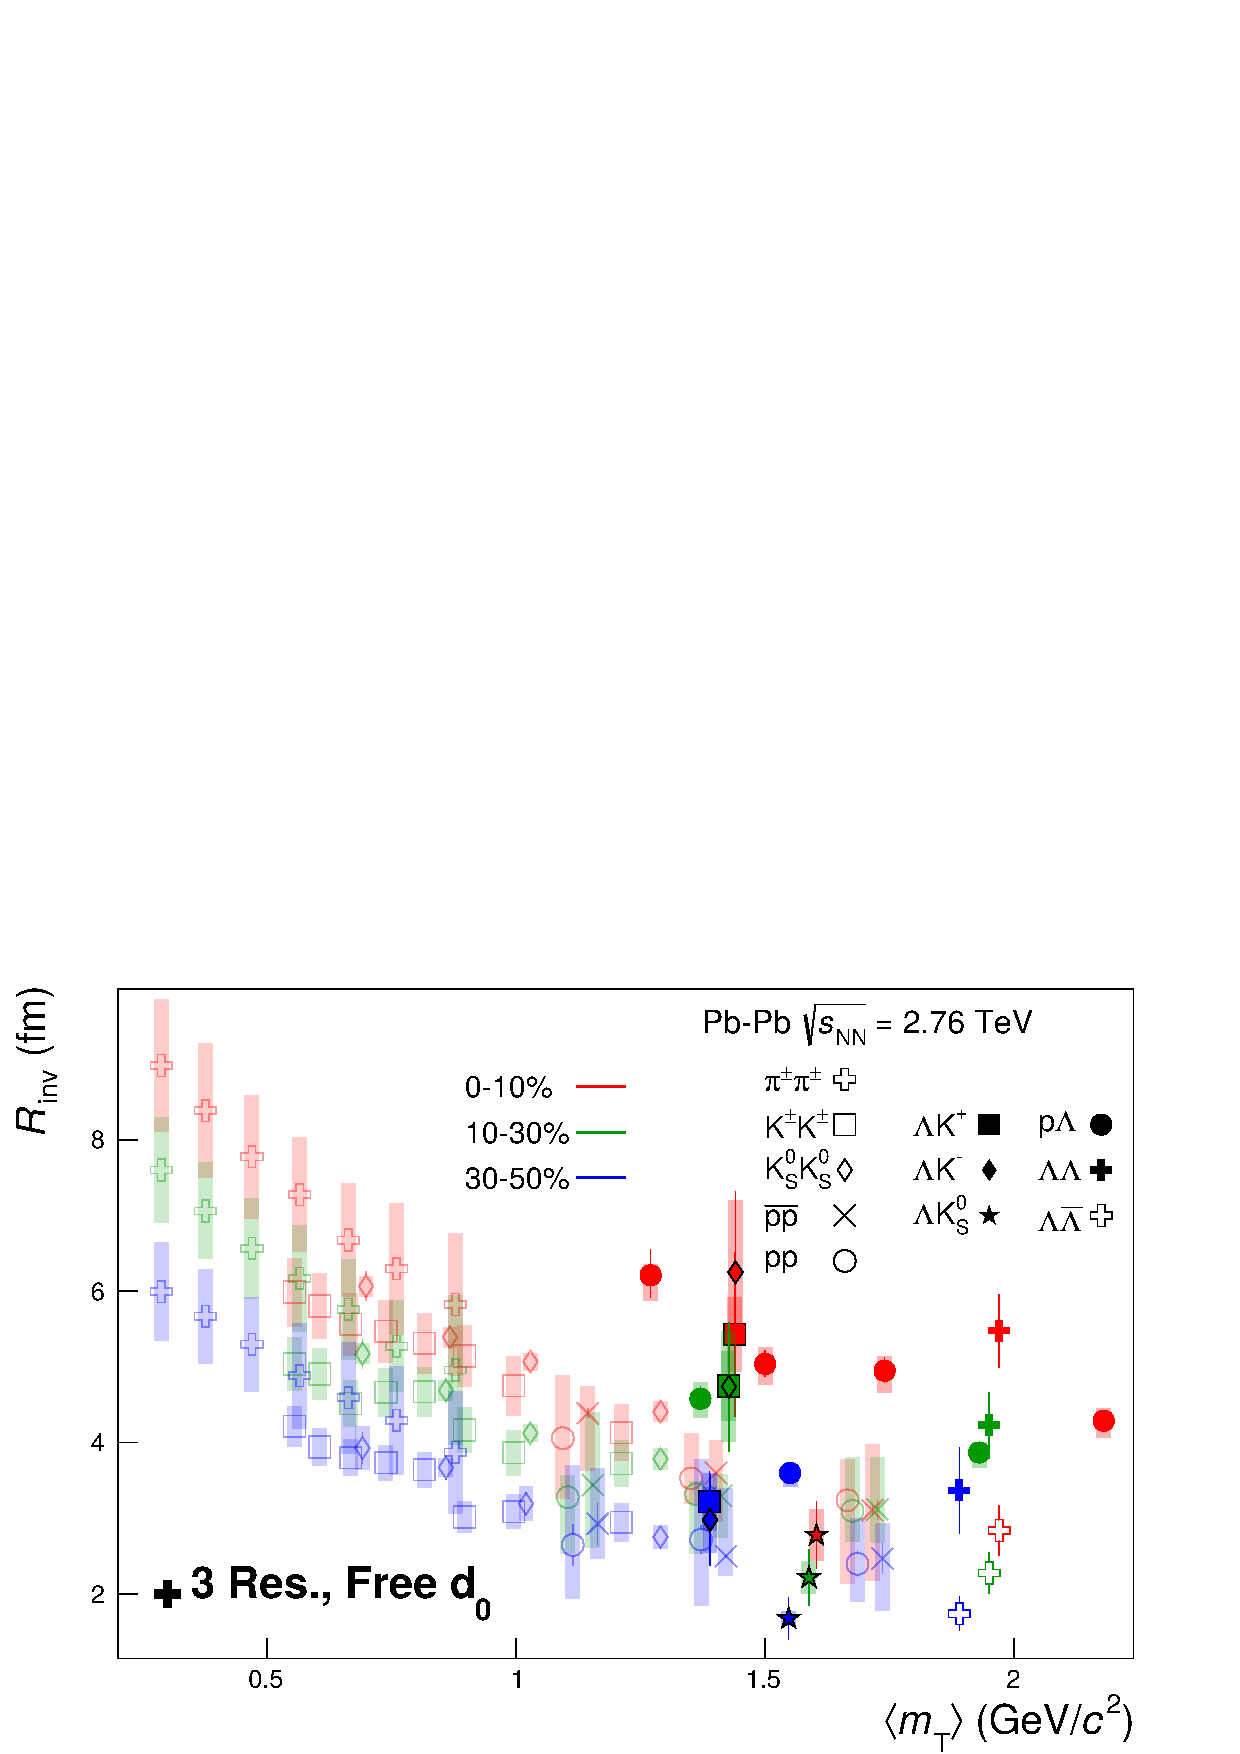
\includegraphics[width=\textwidth]{7_ResultsAndDiscussion/Figures/mTscaling_MinvCalc_OutlinedPoints_OthersTransparent_3Res_FreeD0.pdf}
  \caption[$m_{\mathrm{T}}$ Scaling of Radii: 3 Residuals in Fit]{3 residual correlations in $\Lambda$K fits.  Extracted fit $R_{\mathrm{inv}}$ parameters as a function of pair transverse mass ($m_{\mathrm{T}}$) for various pair systems over several centralities. The ALICE published data \cite{Adam:2015vja} is shown with transparent, open symbols.  The new $\Lambda$K results are shown with opaque, filled symbols.  In the left, the $\Lambda$K$^{+}$ (with it's conjugate pair) results are shown separately from the $\Lambda$K$^{-}$ (with it's conjugate pair) results.  In the right, all $\Lambda$K$^{\pm}$ results are averaged.}
  \label{fig:mTScalingOfRadii_3Res}
\end{figure}

\clearpage

\end{document}